\section{Evaluation of real-time interactions between the user and the agent}
\label{sec:eval}

\subsection{Motivation}

We propose in this section an evaluation of real-time user-agent interactions between an agent controlled by our turn-taking model and a user. We want to measure the effect of the variability of turn-taking strategies of our agent on the user experience of the interaction, especially regarding their comfort level interacting with the agent, or the credibility of the latter. We also want to assess the capacity of our model to coordinate its turns with the user by evaluating the user's judgement on the ability of the agent to take into account the behavior of its partner. The majority of the existing turn-taking models are evaluated solely on performance metrics : the authors measure the capacity of the agent to take the turns after the end of turn of the user, avoiding overlaps while having the most realistic silence duration between the user and the agent \cite{jonsdottir_distributed_2013}. These approaches make the implicit assumption that a better performance is linked to a more credible agent and a better user's engagement. However, having a model able to handle both conflicting situations and smooth transitions with variable durations depending on the motivation of the agent, applying such performance metrics are inappropriate, and we need to find other ways to evaluate our model. 

Some studies have studied the effect of different turn-taking strategies on the user impressions about the agent. \cite{ter_maat_how_2010} propose a wizard of oz experiment where the user is in charge to answer to the questions of the agent. The agent ask one question after another independently of what the user says and vary the moment where the agent starts asking the next question : begin to speak slightly before the end of turn of the user, begin to speak just after the user's end of turn, and begin to speak after a moment of silence lasting a few seconds. The perception the user has about the agent is evaluated by questionnaires with questions linked to the agent's personality and its social skills. \cite{skantze_towards_2010} and \cite{de_vault_toward_2015} elaborated two experiments aiming at evaluating dialogical interactions in the context of mixt-initiative scenarios. In these two experiments, the agents were at least partially controlled by a wizard of oz. In \cite{skantze_towards_2010}, only the user's utterances were transcribed by the wizard of oz, the remaining being managed by the system, and in \cite{de_vault_toward_2015}, the whole step from interpretation to generation was managed by a wizard of oz. In these two interactions, the interaction is both evaluated by questionnaires about the user's satisfaction, the ease of interacting with the agent and the presence of akward silences in the conversation and objective measures linked to transition durations and interruptions are also realized and compared to human interactions for \cite{de_vault_toward_2015}. 

\subsection{Protocol}

We propose to compare our turn-taking model with an implementation of a second model.In this second model, the agent's turn-taking abilities are controlled by simple rules were the agent consider the user has taken turn after a certain amount a silence following the moment the user stopped speaking, and systematically interrupt when the user overlap with the agent. These kind of control strategies are often employed in spoken dialog systems and agents architectures, and considered as non-optimal \citep{ward_root_2005}. For this model, we use the silence threshold value usually used to decide whether the user has finished his turn or not, that is 600 ms, and detect the beginning of turn of the user 100 ms after having detected the voice of the user. We compare this implementation with our current turn-taking model where the agent varies its motivation to change or not role over the conversation. In order to systematize the variations of turn-taking strategies along the conversation, we chose to divide the interaction between the participants in two part : in the first part, the agent has a weak motivation to speak, that is, a weak motivation to keep its role as a speaker, resulting in an agent that will likely pause when the user interrupts it and a weak motivation to change role as a listener, resulting in an agent that will likely wait the user's end of turn before taking turn. In the second part, the agent has a strong motivation to speak, implying that the agent will likely not wait the user's end of turn to begin speaking, often interrupting it, and will likely keep the turn in response to user barge-ins. In the following we will name the condition were the agent is controlled by our model ``condition 1" composed of two conditions, ``condition 1 weak", where the agent has a weak motivation to speak and ``condition 1 strong" where the agent has a strong motivation to speak. The condition corresponding to the control of speaking turns by temporal thresholds is called ``condition 2". For user-agent interaction, we employed a negociation scenario similar to the scenario we used to collect a corpus of human interactions described in \cite{jegou_continuous_2015}. In this scenario, both participants are on a sinking boat, and prepare to embark on a life boat. Each participants has different beliefs on their situations : one think that they are close to the coast, its priority is then to go to the coast the more rapidly possible, the other think he is far from the coast, its priority being then to survive as long as possible. Given their different beliefs, they had to agree about three objects to embark with them in the life boat among six. Moreover participants have at the beginning of the interaction, the knowledge of three possible objects to embark with him and has to discover the other possible objects by asking to its interlocutor. In the actual user-agent scenario, the user believes that they are close to the coast and the agent believes that they are far from the coast. In order to let the user freely interaction with the agent, the interpretation and determination of the utterance said by the agent is realized by a wizard of oz. The latter interprets the user's sentence and decide what is the most appropriate sentence to pronounce. To evaluate some differences between both models, for example linked to the timing of turn transitions by the agent, we needed the wizard to be able to rapidly choose the utterance to generate before the user finished to talk. Once the utterance chosen by the wizard it is the responsibility of the turn-taking model to determine when to run the sentence. In order to permit the agent to rapidly select the utterance, we elaborated the interface shown in the figure ... .
This interface is divided in four parts. The first part is composed of different buttons that the wizard choose to determine the next utterance. The utterance commands are organized as a tree, the top of the tree contains utterances that refers to the beliefs the agent has about his current situation (``Far from the coast"). Given this belief, the agent has several desires linked to this belief, theses desires compose the second layer of command. In our example, if the agent thinks he is far from the coast, he will want to have object that permits to feed for several weeks and stay warm. Under the desire commands are the utterance designing objects that permit to fulfill the different desires of the agent. To each bouton is associated several utterances that permit to vary the utterances produced by the agent. The utterances generated by our agent are all utterances collected from a corpus of human interactions. 
The interface possess also buttons generating counter-arguments linked to the beliefs, desires and objects proposed by the user. 
Moreover, the agent has the possibility to generate backchannels, responses to yes-no questions, feedbacks showing its agreement or desagreement and short utterances asking the user to repeat what he said.
The control of the agent's motivation has been automated, such as, for the first condition, the motivation value change after half of the interaction that is 1 min 15 s. The agent has two possible motivation values, a weak motivation, $m=0.4$ and a strong motivation value $m=1.0$. Each participant interacted two times with the agent, each time with a different condition and according to the same scenario. For each condition, the interaction lasted 2 min 30 s. At the end of each interaction, a questionnaire was proposed to the participants comprising questions about the satisfaction to interact with the agent, the ease with wich the participant interacted with the agent and its perception about the intentionality of interruptions by the user, that is whether the interruptions made by the agent were due to an agent mistakenly perceiving the end of turn of the user or whether the agent interrupted on purpose. In this questionnaire, different assertion were made for which the participant had to write its level of agreement, between strongly disagree and strongly agree in a continuous scale between 0 à 10. The different affirmations were inspired from \cite{skantze_towards_2010}, \cite{bevacqua_effects_2014} and \cite{de_vault_toward_2015}.

\subsection{Results}

31 volonteers (30 men and 1 woman) participated to the experiment. They were all native french speakers and were students, engineers or researchers. The results to the questionnaire are shown on the table \ref{Answers}. 
\begin{table}
\centering
\resizebox{\linewidth}{!}{\begin{tabular}{|p{3cm}|p{2cm}|p{2cm}|p{2cm}|}
\hline
Question & Median cond. 1 & Median cond. 2 & p-value \\
\hline
My interlocutor \linebreak didn't perceive the moment were I talked & 2.25 & 1.75 & 0.95\\
\hline
My interlocutor took the turn randomly& 2.5 & 2.625 & 0.6 \\
\hline
My interlocutor interrupted unvolontarily& 6 & 4 & 0.019* \\
\hline
My interlocutor interrupted me on purpose& 6 & 6.5 & 0.91 \\
\hline
My interlocutor paid attention not to interrupt me & 4.5 & 7.5 & 0.006**\\
\hline
My interlocutor was slow to respond to me & 3 & 2 & 0.77\\
\hline
My interlocutor refused sometimes to speak to me & 6.125 & 5.75 & 0.16\\
\hline
My interlocutor annoyed me by the way he took the turn & 4.5 & 3.25 & 0.54\\
\hline
I was at ease interacting with my interlocutor & 5.25 & 6.25 & 0.55\\
\hline
I liked speaking with my interlocutor & 6.625 & 7 & 0.52\\
\hline
The behavior of my interlocutor was close to the behavior of a human speaker & 5.625 & 6.5 & 0.97\\
\hline
\end{tabular}}
\caption{Assertions and answers for the conditions 1 and 2.}
\label{Answers}
\end{table}

In this table are translated the different assertions of the question, the mean responses of the participants, and the significance of differences in the responses between the two conditions. The participants liked speaking with the agent. The results of the questions related to the credbility of the agent are more mitigated, with participants with a median value to the assertion "The behavior of my interlocutor was clode to the behavior of a human speaker" of 6.5 in the second condition and 5.625 in the first condition. The users perceived that the agent paid more attention not to interrupt them (median value of 7.5) for the second condition than for the first condition. Nevertheless, participant perceived also counter-intuitively that the agent interrupted them more unvolontarily in the first condition compared to the second condition, even if the degree of agreement with the assertion "My interlocutor interrupted me unvolontarily" did not strongly favorized this assertion (median of 6). The fact that the participants considered that their interlocutor interrupted them unvolontarily in the first condition is problematic. We should note that the number of overlaps initiated by the agent is much greater than what we expected : indeed, this number is not significantly depending on being in the condition 1 or being in the condition 2.

We completed the analysis of the subjective evaluations with an objective analysis of the interaction? We first analyzed the transition durations between the different conditions (condition 1 Weal, condition 1 Strong, condition 2), separating user to agent transitions from agent to user transitions. For the analysis of transition durations, we annotated manually the turns of the different participants and aligned the loudness profile of the participants to the annotations we made. We kept only transitions that were not overlaps and transitions that were not anticipated by the agent. We observed first a high number of mistakes in the detection of user end of turns in conditions 1 and 2, with almost 50 \% of transitions having at least slight overlaps.  The repartition of the user to agent transitions is shown on figure \ref{box_ua}, and the repartition of agent to user transitions is shown on the figure \ref{box_au}. 

\begin{figure}
\centering
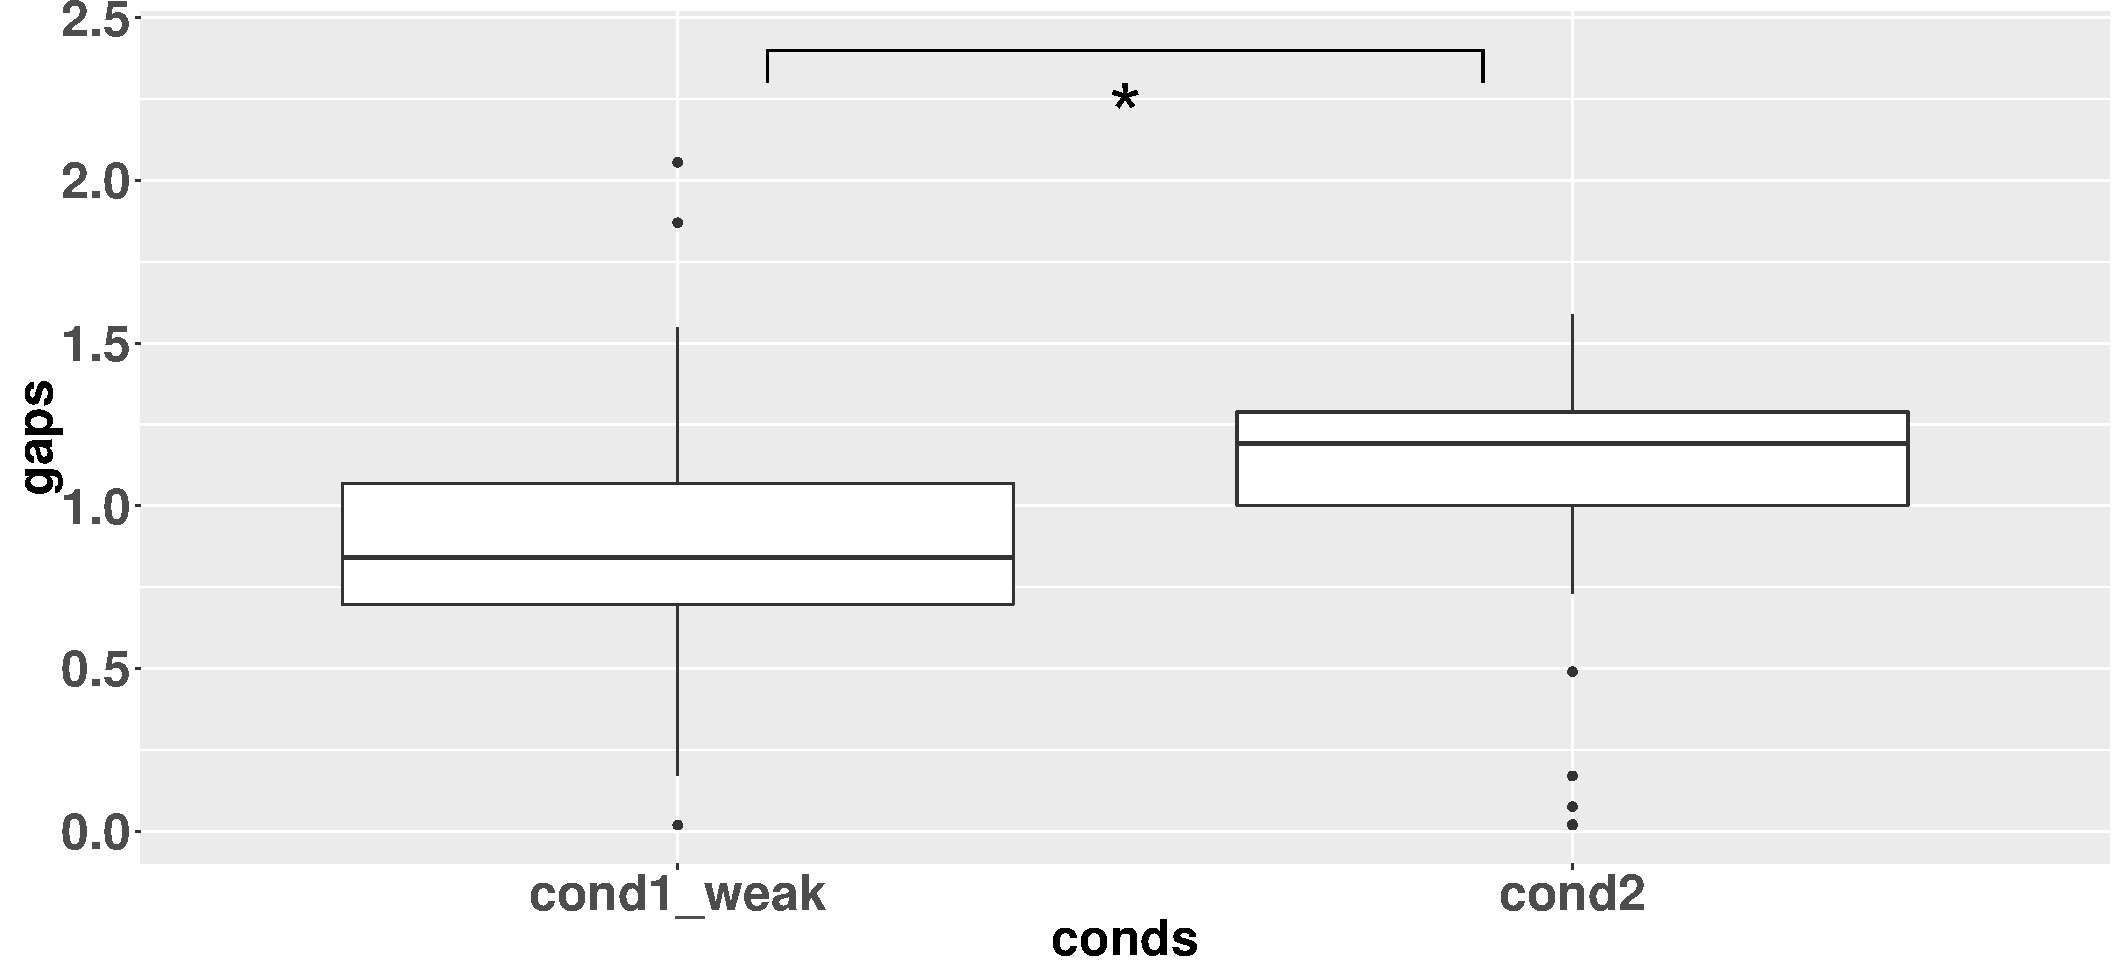
\includegraphics[width=\linewidth]{figure/boxTransitionsUA.pdf}
\caption{Repartition of user to agent silence durations during transitions}
\label{box_ua}
\end{figure}

\begin{figure}
\centering
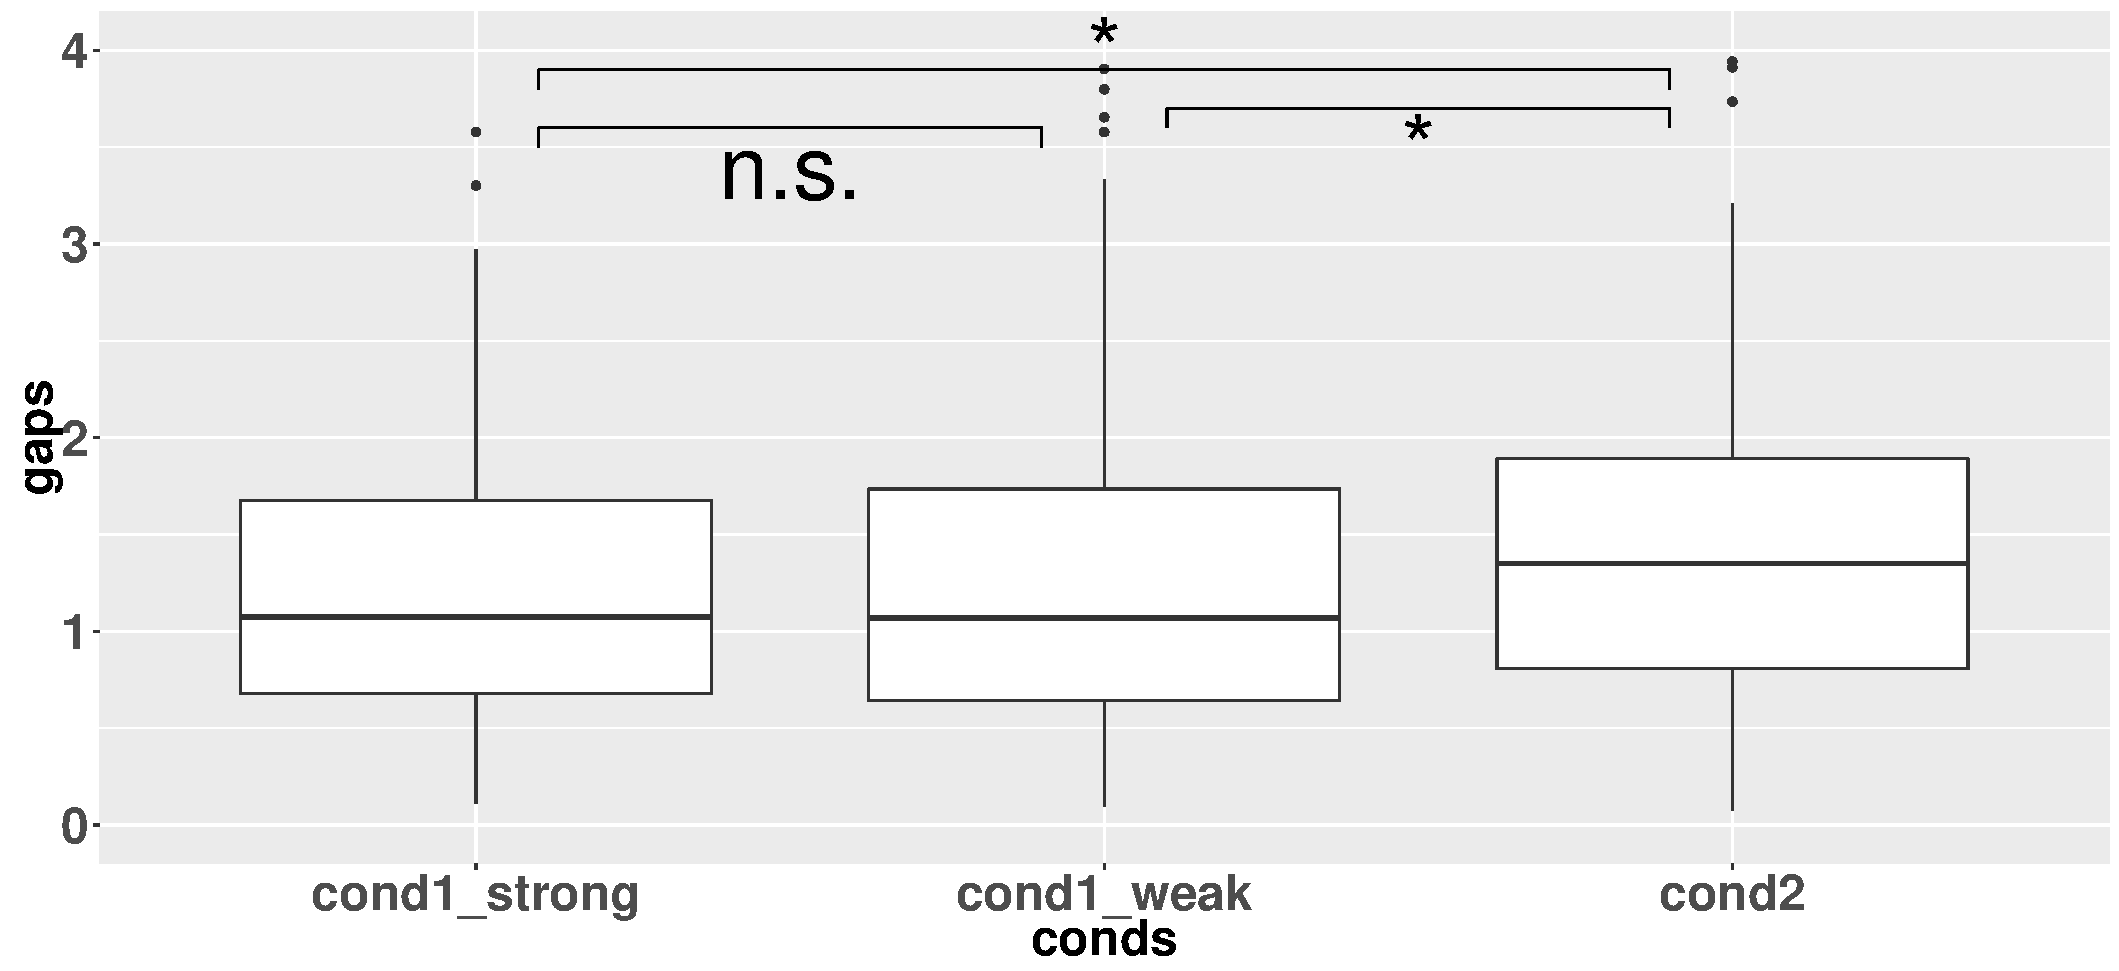
\includegraphics[width=\linewidth]{figure/boxTransitionsAU.pdf}
\caption{Repartition of agent to user silence durations during transitions}
\label{box_au}
\end{figure}

These results show that for the condition 1 the agent takes the turn more rapidly (840 ms in mean) compared to the second condition (1.19 s in mean), the difference in the silence durations between these two conditions being significant (p<0.05), and the same principle apply for agent-user transitions, the mean silence duration before the user takes the turn being 1.11 s for the first condition and 1.39 s for the second condition with a significant difference between the two conditions (p<0.05). 
In addition to these transition duration values, the pitch variation of the participants was measured during interruptions by the agent. The results showed that the pitch of the user was significantly greater than the mean pitch of the participant during conflictual moments, for the condition 1 ``Strong".

% Comment peut-on expliquer que la durée moyenne de transition soit le double du seuil de détection de la fin de tour de l'utilisateur ?
% À faire : valeur moyenne de pitch supérieure aussi lors des overlaps de l'agent pour les autres conditions, différences de perception qui pourrait laisser penser une différence de traitement ?
% Comportement de l'agent : est-ce que l'utilisateur a beaucoup interrompu l'agent ?


\subsection{Discussion}

The results of our questionnaire doesn't seem to show effects on the variations of the turn-taking behaviors on the impressions the user had on the interaction. The results of the questionnaire were compared to beahvioral analysis showing that the user produced a significant but weak reaction when the agent interrupted the user, but when varying the way the agent took turn (waiting the end of the user's turn or interrupting the user) between the conditions 1 ``weak" and 1 ``strong" we did not find modifications of the silence duration of agent to user transitions. At the end of the experiment, we collected the oral impressions of the participants on the interaction. Participants reported less categorical impressions towards the interruptions of the user than what has been observed in the responses of the questionnaires. Six participants explicitly mentionned that they perceived the interruptions of the agent as non-voluntary, on the oppsite, thirteen participants perceived at least some interruptions as voluntary. Among these thirteen participants, four participants judged these interruptions as coherent and credible given the dialog context, and five participants associated these interruptions to the fact that the agent did not agree or tried to impose its own ideas. Finally, among those thirteen participants, five participants judged those interruptions as humanlike. Nevertheless, these perception of the interruption did not conducted to more positive impressions about the interaction such a increasing naturality or credibility. One of the participants we interviewed after the experiment reported a rage feeling linked to the incessant interruptions of the agent, and two participants reported that they were annoyed by these interruptions. The results of the questionnaire have also shown that the subjects perceived the agent as strongly reactive and have scarcely noticed the presence of awkward silences during the conversation. When these moments of silence were perceived, they were considered as not natural, even if two participants perceived it as credible and linked to an agent that thought at what it wanted to say. This non natural character of awkward silences could be linked to the fact that the interaction was only audio preventing the agent to provide visual feedback to the user. 
The high rate of end of turn detections by the two models (50 \% of user-agent transitions) can partially explained by the voice activity detector used to detect the moments were the user spoke, showing an important number of moments were no voice was detected whereas the user actually spoke. The fact that the participants seemed not disturbed by the relatively high silence duration of user to agent transitions support the idea that the latter does not expect optimal turn transitions from the agent. The reports collected from the interviews of the participants tend to show that those interruptions can give an impression of smoothness and immersion in the dialogue, but, as the participants often mentionned the interruptions of the agent related to the dialog, to the condition that the interruption should be coherent to the dialog context and what the agent has to say. Finally, the lack of distinction between interruptions, those that were due to mistakes in the detection of the user end of turn and those that were voluntary could be due to difficulties of the participants to perceive the prosodic variations of the agent. These difficulties could come from the quality of the tts voice we used, participants having often reported the bad quality of the voice. 

